
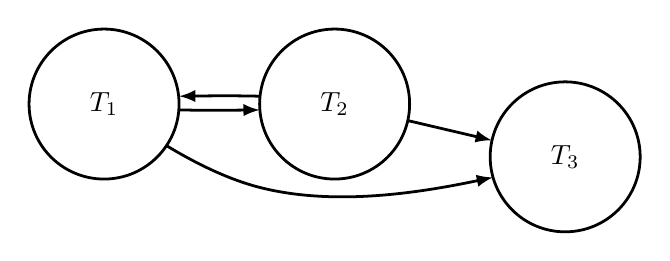
\begin{tikzpicture}[>=latex,line join=bevel,]
  \pgfsetlinewidth{1bp}
%%
\pgfsetcolor{black}
  % Edge: T_1 -> T_2
  \draw [->] (54.075bp,43.882bp) .. controls (60bp,43.769bp) and (66.4bp,43.729bp)  .. (82.974bp,43.883bp);
  % Edge: T_2 -> T_3
  \draw [->] (136.63bp,39.988bp) .. controls (142.89bp,38.519bp) and (149.71bp,36.919bp)  .. (166.54bp,32.973bp);
  % Edge: T_2 -> T_1
  \draw [->] (82.974bp,48.823bp) .. controls (77.051bp,48.974bp) and (70.653bp,49.028bp)  .. (54.075bp,48.824bp);
  % Edge: T_1 -> T_3
  \draw [->] (49.687bp,30.9bp) .. controls (59.407bp,25.019bp) and (71.301bp,18.983bp)  .. (83bp,16bp) .. controls (107.23bp,9.8208bp) and (135.33bp,12.891bp)  .. (166.96bp,19.599bp);
  % Node: T_2
\begin{scope}
  \definecolor{strokecol}{rgb}{0.0,0.0,0.0};
  \pgfsetstrokecolor{strokecol}
  \draw (110bp,46bp) ellipse (27bp and 27bp);
  \draw (110bp,46bp) node {$T_2$};
\end{scope}
  % Node: T_3
\begin{scope}
  \definecolor{strokecol}{rgb}{0.0,0.0,0.0};
  \pgfsetstrokecolor{strokecol}
  \draw (193bp,27bp) ellipse (27bp and 27bp);
  \draw (193bp,27bp) node {$T_3$};
\end{scope}
  % Node: T_1
\begin{scope}
  \definecolor{strokecol}{rgb}{0.0,0.0,0.0};
  \pgfsetstrokecolor{strokecol}
  \draw (27bp,46bp) ellipse (27bp and 27bp);
  \draw (27bp,46bp) node {$T_1$};
\end{scope}
%
\end{tikzpicture}

